\jxhj{%教学后记
	}
\skrq{%授课日期
	2017年 | 5月9日 |5月16日|5月23日|5月30日|6月7日| 1-3节}
\ktmq{%课题名称
	 薄壁配合件加工}
\jxmb{%教学目标,每行前面要加 \item
	\item 掌握薄壁零件的加工工艺;
	\item 掌握配合件的加工工艺;
	\item 能对零件进行简化编程;
	\item 掌握自动编程的基本知识。}
\jxzd{%教学重点,每行前面要加 \item
	\item 薄壁零件的加工工艺;
	\item 配合件的加工工艺。}
\jxnd{%教学难点,每行前面要加 \item
	\item 配合件的加工工艺。}
\jjff{%教学方法
	通过讲述、举例、演示法来说明;}

\makeshouye %制作教案首页

%%%%教学内容
\subsection{实习教学要求}
\begin{enumerate}[1、]
	\item 握配合零件的加工工艺;
	\item 能对配合零件进行简化编程;
	\item 巩固刀具半径补偿的灵活使用;
    \item 能控制好薄壁零件的加工精度;
    \item 能用~mastercam~生mastercam成程序。
\end{enumerate}


\subsection{相关工艺知识与编程}

\subsubsection{薄壁零件的特点}
1、工具钢性差,容易变形。

2、形状不规则。

3、其材料多为铝合金精密铸造件,无缝钢管,也有采用耐热、耐腐蚀合金。

\subsubsection{薄壁零件的加工}
1、减小精加工时工艺钢性

减小精加工时,薄壁的高度,即粗加工一层,就马上精加工一层,多次换刀。

2、减小切削力

A、选用合理的刀具

B、选用合理的切削用量

主要:减小吃刀深度

粗加工时,提高效率,可增大进给量

精加工时,还可以用增大切削速度来减小切削力。

C、减小切削热

粗加工时,使用水溶液,冷却。

精加工时,使用切削油或高浓度的乳化液

\subsubsection{薄壁零件的编程}

1、使用一个加工轮廓进行编程,(已标尺寸)

2、编写两个独立程序。

3、共用部分程序。(圆弧切入切出)

切入切出写在新的子程序中。

4、用直线切入切出

要有重叠量。

5、多使用简化编程

6、刀补值得计算

考虑薄壁的厚度


\subsubsection{配合件的质量要求}
A.尺寸精度:可用刀具半径补偿进行控制

B.形位精度:精加工时可打开刀具半径速率修调

C.表面质量:选择合理的切削用量

D.配合要求:

过盈配合、间隙配合、过渡配合

保证方法:

一件严格按零件尺寸加工, 相关尺寸要作相应的处理,

如取中值或极限值

另一件则配做, 直到满足配合要求为止,

也可严格按其加工零件进行加工,再进行修正.

\subsubsection{配合的编程处理}
配合部分的轮廓一般是相同的。

它们可以共用同一个轮廓子程序。

再使用不同的刀具半径补偿控制精度

对于开放的轮廓,给刀补及切入切出可放在轮廓子程序中

对于封闭的轮廓,给刀补及切入切出可放在上级子程序中

如不用圆弧切入切出,切入切出要有重合量。


\subsection{实习内容及过程}

\subsubsection{集合、组织实习}
1、清查学生人数

2、文明安全生产讲解

3、实习内容说明
\subsubsection{开机15分钟}
1、由组长记录机床相关问题

2、开机前检查仔细

3、空转几分钟预热
\subsubsection{机床操作及编程}
1、教师演示基本操作

2、组长安排2人员操作机床(1人操作,1个指导)

3、其他人员自选图形编程

4、每人操作时间不得超过2小时

5、教师巡回指导
\subsubsection{操作点评及工件检测}
1、学生操作感想说明及自评

2、教师提问及点评

3、学生对工件自测

4、教师检测及评分
\subsubsection{准备下课}
1、清洁数控机床

2、正常关机

3、集合教师点评

\subsection{练习题及作业}
\begin{figure}[!hbtp]
	\centering	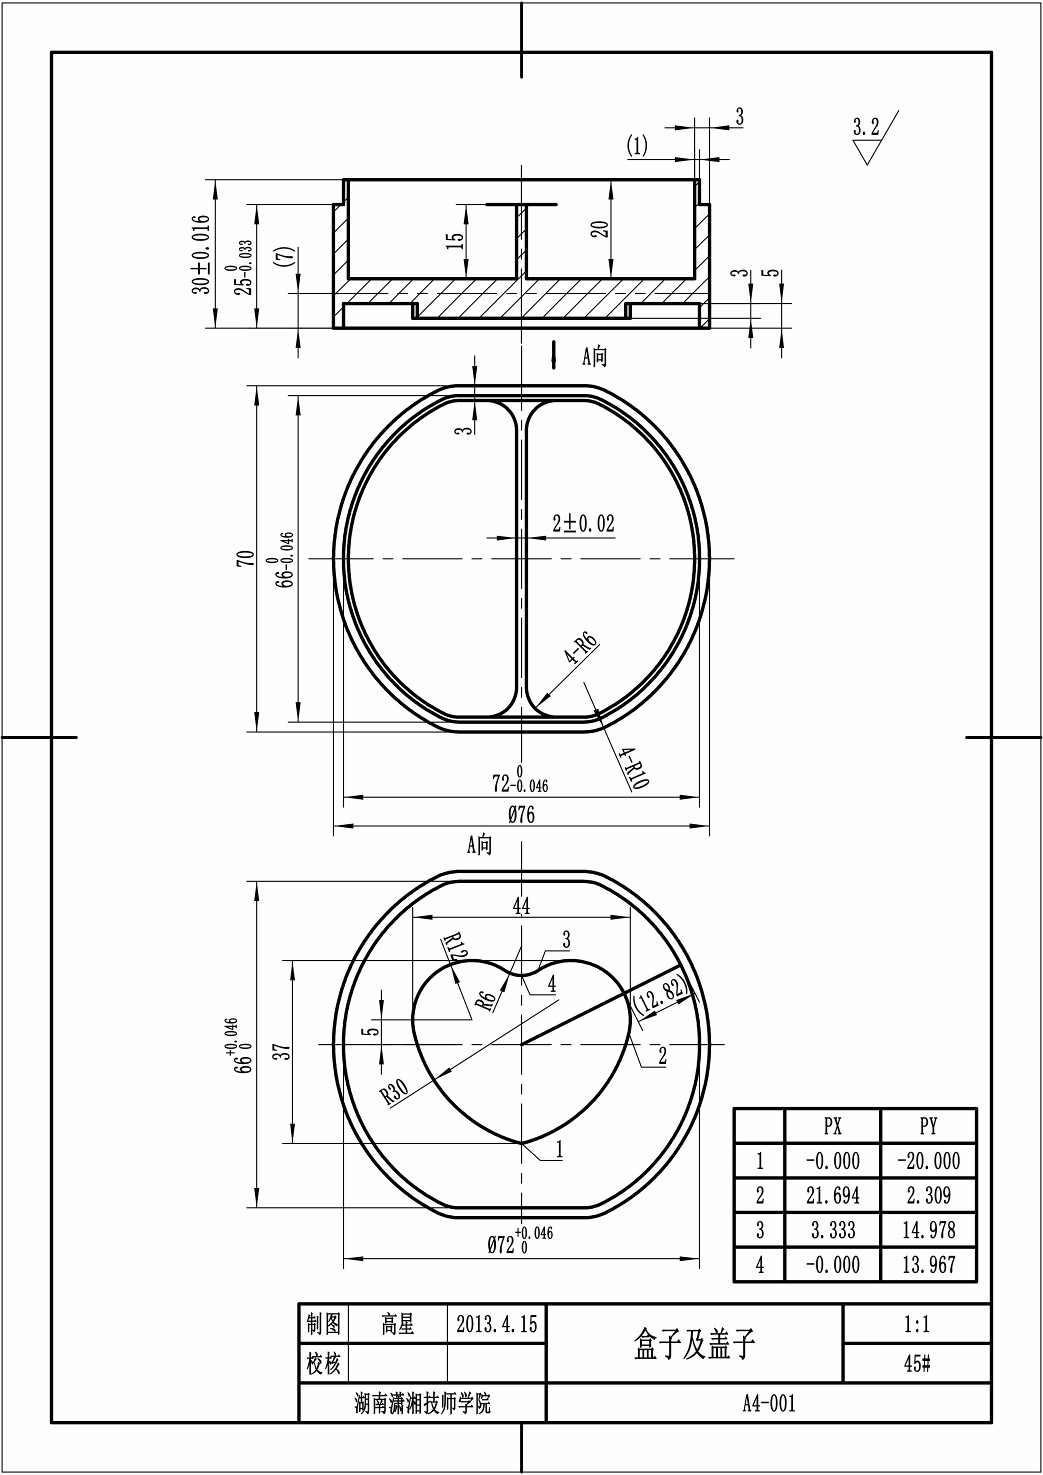
\includegraphics[width=0.9\textwidth]{images/shixi_4-1}
	\caption{薄壁配合件} \label{薄壁配合件}
\end{figure}

\vfill
\subsection{加工准备与加工要求}
\subsubsection{加工准备}
\begin{enumerate}[1、]
	\item 设备:数控铣床、加工中心。
	\item 材料:45圆钢(Ф110*35)。
	\item 工具:活动扳手,平行垫铁,百分表,其它常用辅具。
	\item 量具:外径千分尺(0~25、100~125,0.01),深度千分尺(0~25,0.01),R规。
	\item 刀具:Ф10、Ф16、Ф14立铣刀、Ф64面铣刀。
	\item 夹具:三爪自定心卡盘、螺杆压板、平口钳。
\end{enumerate}
\subsubsection{课题评分表}

{\noindent
%\begin{figure}[!hbtp]
%	\centering	
\footnotesize
\hspace{-2.8ex} \renewcommand\arraystretch{1.9}
\begin{tabu} to 0.5\textwidth {|cc|c|c|c|c|c|c|}
	\hline 
	\multicolumn{2}{|c|}{工件编号}  &\multicolumn{2}{c}{} & \multicolumn{2}{|c}{总得分}   & \multicolumn{2}{|c|}{ }   \\ 
	\hline 
	\multicolumn{2}{|c|}{项目与配分} &\parbox{2ex}{序号}  & 技术要求 & 配分 & 评分标准 &  \parbox{4ex}{检测记录}& 得分 \\ 
	\hline 
	\multirow{4}{*}{ \parbox{4ex}{工件加工 (80)}} &\multicolumn{1}{|c|}{上面}  & 1 &面铣  & 4 & 超差全扣 & & \\ 
	\cline{2-8}  
	&\multicolumn{1}{|c|}{上面}   & 2 &尺寸1  & 12 & 超差全扣 & & \\ 
	\cline{2-8} 
	&\multicolumn{1}{|c|}{上面}  & 3 &尺寸2  & 12& 超差全扣 & & \\ 
	\cline{2-8} 
	&\multicolumn{1}{|c|}{上面}   & 4&椭圆  & 30 & 超差全扣 & & \\ 
	\hline 
	\multicolumn{2}{|c|}{\multirow{2}{*}{\parbox{10ex}{程序与工艺
				(10\%)} } }&5  &程序正确合理  & 5 & 每错一处扣2分 &  &  \\ 
	\cline{3-8} 
	&&6&加工工序卡  &5  &不合理每处扣2分  &&  \\ 
	\hline 
	\multicolumn{2}{|c|}{\multirow{2}{*}{\parbox{10ex}{机床操作
				(10\%)}
	} } &7 &机床操作规范  & 5 & 出错一次扣2分 &  &  \\ 
	\cline{3-8} 
	&&8&工件刀具装夹  &5  &出错一次扣2分&&  \\ 
	\hline 	
	\multicolumn{2}{|c|}{\multirow{2}{*}{\parbox{10ex}{安全文明生产
				(倒扣分)}
	} } &9  &安全操作  & 倒扣 & \multirow{2}{*}{\parbox{14ex}{安全事故停止操作或酌情扣分}}&  &  \\ 
	\cline{3-5} \cline{7-8} 
	&&10&机床整理  &倒扣  &  &  &\\ 
	\hline 	
\end{tabu} }
%\end{figure}
\vfill